\begin{frame}{Dataset Overview}
 \begin{center}
    \begin{figure}
    \centering
     \begin{tikzpicture}
        % Sample image and dimensions
         \node[visible on=<1->, step_rectangle] at (0,5.9) (sample) {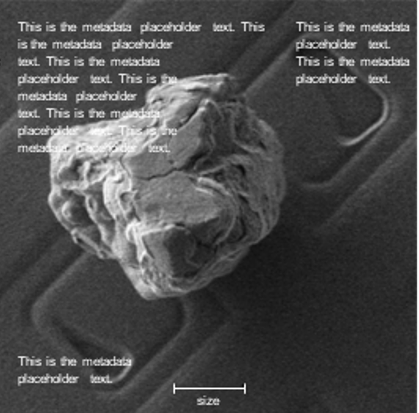
\includegraphics[scale=0.4]{sample_defect.png}};
        \draw[decoration={mirror,raise=3mm},decorate] (-2.6,8.2) -- (-2.6,3.6) node[left,midway] {480};
        \draw[decoration={mirror,raise=-3mm},decorate] (-2.3,3.33) -- (2.3,3.33) node[below,midway] {480};

        % Metadata boxes
        \node[visible on=<2->, right=\imgfinal of sample, step_rectangle, xshift = 1.5cm, yshift = 1.5cm] (firstrectcenter) {Technology};
        \node[visible on=<2->, left=\img of firstrectcenter, step_rectangle] (firstrectleft) {...};
        \node[visible on=<2->, right=\img of firstrectcenter, step_rectangle] (firstrectright) {...};
        
        \node[visible on=<3->, right=\imgfinal of sample, step_rectangle, xshift = 1.65cm, yshift = 0cm] (secondrectcenter) {Product};
        \node[visible on=<3->, left=\img of secondrectcenter, step_rectangle] (secondrectleft) {...};
        \node[visible on=<3->, right=\img of secondrectcenter, step_rectangle] (secondrectright) {...};
        
        \node[visible on=<4->, right=\imgfinal of sample, step_rectangle, xshift = 1.5cm, yshift = -1.5cm] (thirdrectcenter) {Step/Layer};
        \node[visible on=<4->, left=\img of thirdrectcenter, step_rectangle] (thirdrectleft) {...};
        \node[visible on=<4->, right=\img of thirdrectcenter, step_rectangle] (thirdrectright) {...};

        %  Arrows
        \draw[visible on=<3->, arrow_small] (firstrectcenter) -- (secondrectcenter);
        \draw[visible on=<3->, arrow_small] (firstrectcenter) -- (secondrectleft);
        \draw[visible on=<3->, arrow_small] (firstrectcenter) -- (secondrectright);
        
        \draw[visible on=<4->, arrow_small] (secondrectcenter) -- (thirdrectcenter);
        \draw[visible on=<4->, arrow_small] (secondrectcenter) -- (thirdrectleft);
        \draw[visible on=<4->, arrow_small] (secondrectcenter) -- (thirdrectright);
        
     \end{tikzpicture}
     \caption*{\hspace*{4em} Image dimensions. \uncover<2->{\hspace*{7em} Correlated metadata.}}

     \end{figure}
 \end{center}
\end{frame}

\begin{frame}{Dataset Distribution}
  \begin{figure}[h]
    \centering
        \resizebox{8cm}{4.5cm}{
        \begin{tikzpicture}[font=\small]
            \pgfplotsset{every axis/.append style={
                axis x line=middle,    % put the x axis in the middle
                axis y line=middle,    % put the y axis in the middle
                axis line style={-}, % arrows on the axis
                label style={font=\small},
                tick label style={font=\tiny},
                },}
            \begin{axis} [ybar,
              bar width=3.1mm,
              ymin=0,
              ymax=1500,
              xtick=data,
              axis x line=bottom,
              axis y line=left,
              enlarge x limits=0.02,
              x=0.31cm,
              ylabel={Samples}, 
              xlabel={Label},
              x label style={at={(axis description cs:0.5,-0.1)},anchor=north},
              y label style={at={(axis description cs:-0.05,.5)},rotate=90,anchor=south},                    
              ]
              \only<2->{\draw[dashed, maincolor] (axis cs:0, 500) -- (axis cs:37.5, 500);}
              \only<1>{\addplot[scatter,scatter src=y,mark=ybar, fill = plotcolor, draw=maincolor] coordinates {
                (1,441)
                (2,136)
                (3,168)
                (4,415)
                (5,1492)
                (6,1410)
                (7,58)
                (8,309)
                (9,85)
                (10,95)
                (11,174)
                (12,375)
                (13,156)
                (14,408)
                (15,190)
                (16,286)
                (17,337)
                (18,477)
                (19,101)
                (20,372)
                (21,659)
                (22,630)
                (23,256)
                (24,50)
                (25,168)
                (26,52)
                (27,988)
                (28,209)
                (29,830)
                (30,212)
                (31,168)
                (32,92)
                (33,83)
                (34,51)
                (35,417)
                (36,131)
                (37,128)
              };}
              \only<2>{\addplot[scatter,scatter src=y,mark=ybar, fill = plotcolor, draw=maincolor] coordinates {
                (1,441)
                (2,136)
                (3,168)
                (4,415)
                (5,1492)
                (6,1410)
                (7,58)
                (8,309)
                (9,85)
                (10,95)
                (11,174)
                (12,375)
                (13,156)
                (14,408)
                (15,190)
                (16,286)
                (17,337)
                (18,477)
                (19,101)
                (20,372)
                (21,659)
                (22,630)
                (23,256)
                (24,50)
                (25,168)
                (26,52)
                (27,988)
                (28,209)
                (29,830)
                (30,212)
                (31,168)
                (32,92)
                (33,83)
                (34,51)
                (35,417)
                (36,131)
                (37,128)
              };}
              \only<3>{\addplot[scatter,scatter src=y,mark=ybar, fill = plotcolor, draw=maincolor] coordinates {
                (1,441)
                (2,136)
                (3,168)
                (4,415)
                (5,500)
                (6,500)
                (7,58)
                (8,309)
                (9,85)
                (10,95)
                (11,174)
                (12,375)
                (13,156)
                (14,408)
                (15,190)
                (16,286)
                (17,337)
                (18,477)
                (19,101)
                (20,372)
                (21,500)
                (22,500)
                (23,256)
                (24,50)
                (25,168)
                (26,52)
                (27,500)
                (28,209)
                (29,500)
                (30,212)
                (31,168)
                (32,92)
                (33,83)
                (34,51)
                (35,417)
                (36,131)
                (37,128)
              };}
              \only<4>{\addplot[scatter,scatter src=y,mark=ybar, fill = plotcolor, draw=maincolor] coordinates {
                (1,500)
                (2,500)
                (3,500)
                (4,500)
                (5,500)
                (6,500)
                (7,500)
                (8,500)
                (9,500)
                (10,500)
                (11,500)
                (12,500)
                (13,500)
                (14,500)
                (15,500)
                (16,500)
                (17,500)
                (18,500)
                (19,500)
                (20,500)
                (21,500)
                (22,500)
                (23,500)
                (24,500)
                (25,500)
                (26,500)
                (27,500)
                (28,500)
                (29,500)
                (30,500)
                (31,500)
                (32,500)
                (33,500)
                (34,500)
                (35,500)
                (36,500)
                (37,500)
              };}
              
              \end{axis}
        \end{tikzpicture}
        }\hspace*{1em}
    \only<1>{\caption*{Initial defect class distribution.}}
    \only<2>{\caption*{Initial defect class distribution.}}
    \only<3>{\caption*{Downsampled defect class distribution.}}
    \only<4>{\caption*{Resampled (upsampled \& downsampled) defect class distribution.}}
    \end{figure}
\end{frame}
    
\begin{frame}{Data Augmentation}
    \begin{table}[h]
        \noindent
        \makebox[\linewidth]{
          \centering
          \begin{tabular}{SSS}
          \toprule
          {\textbf{Name}} & {\textbf{Description}} & {\textbf{Value}}   \\ \midrule
          {Horizontal flip}  & {Mirror the image on the x-axis}              & {\{True, False\}} \\ 
          {Vertical flip}    & {Mirror the image on the y-axis}              & {\{True, False\}} \\
          {Rotation}         & {Rotate the image with respect to its center} & {$[-90, 90]$}\\ 
          {Zoom}             & {Zoom in} & {$[1, 1.3]$} \\ 
          {Horizontal shift} & {Shift the image horizontally}                & {$[-0.5, 0.5]$} \\
          {Vertical shift}   & {Shift the image vertically}                  & {$[-0.5, 0.5]$} \\
          \bottomrule
          \end{tabular}
          }
          \caption{Transformations applied to images\label{table:transformations}}
    \end{table}
\end{frame}

\begin{frame}{Backbone Architecture: ResNet50}
    j
\end{frame}